\documentclass[12pt]{article}

% --- Packages ---
\usepackage[utf8]{inputenc}
\usepackage[T1]{fontenc}
\usepackage[french]{babel}
\usepackage{amsmath, amssymb}
\usepackage{geometry}
% \usepackage[draft]{graphicx}
\usepackage{tikz}
\usepackage[most]{tcolorbox}
\usepackage{multicol}
\usepackage{lmodern}
\usepackage{pgfplots}
\pgfplotsset{compat=1.18}
\usepackage{mdframed}
\usepackage{tkz-tab}
\usepackage{bm}
\usepackage{xcolor}
\usepackage{sectsty}
\usepackage[utf8]{inputenc}
\usepackage[T1]{fontenc}
\usepackage[inline]{enumitem}
\usepackage[dvipsnames]{xcolor}
\usepackage{multido}
% --- Page ---
\geometry{margin=2cm}

% Footer
\usepackage{fancyhdr}
\pagestyle{fancy}
\cfoot{\thepage}
\rfoot{\textit{G.M.}}
\renewcommand{\headrulewidth}{0pt}
\renewcommand{\footrulewidth}{0pt}

% Commande pour afficher une image même en mode draft
\newcommand{\showthisimage}[2][]{%
  \let\oldincludegraphics\includegraphics%
  \renewcommand{\includegraphics}[2][]{\oldincludegraphics[##1]{##2}}%
  \includegraphics[#1]{#2}%
  \renewcommand{\includegraphics}[2][]{}%
}

% Pour les normes : 
\newcommand*{\norme}[1]{\left\lVert\overrightarrow{#1}\right\rVert}

\usetikzlibrary{shapes.misc}

\tikzset{cross/.style={cross out, draw=black, minimum size=2*(#1-\pgflinewidth), inner sep=0pt, outer sep=0pt},
%default radius will be 1pt. 
cross/.default={4pt}}

% mettre dans le préambule, après \usepackage{xcolor}
\usepackage{sectsty} % gère facilement la couleur des titres
\setlength{\parindent}{0pt}

\sectionfont{\color{red}\Large\bfseries}     % pour \section*
\subsectionfont{\color{red}\large\bfseries\hspace{1cm}}

\begin{document}

% ============================
%   Variations de fonctions
% ============================

\newpage

\begin{center}
    {\LARGE \textbf{Variations de fonctions}}\\[4mm]
    {\large Seconde}
\end{center}

\hrule
\vspace{0pt}

% ============================
%   PARTIE 1 : Inéquations du premier degré
% ============================

\section*{\textcolor{red}{Partie 1 : Fonctions croissantes et fonctions décroissantes}}

\subsection*{\hspace{1cm} 1) Définition}

On considère en exemple la fonction : $f(x) = 5x - x^2$

\vspace{10pt}
\begin{minipage}[t]{.45\textwidth}%
    \vspace{0pt}
    \begin{center}
        $f$ est \_\_\_\_\_\_\_\_\_\_\_\_ sur \_\_\_\_\_\_\_

        \vspace{10pt}
        Si $x$ augmente ({\color{red}1} < {\color{ForestGreen}2}),

        \vspace{10pt}
        $f(x)$ \_\_\_\_\_\_\_\_\_\_\_\_ (\_\_\_\_\_\_\_\_\_)
        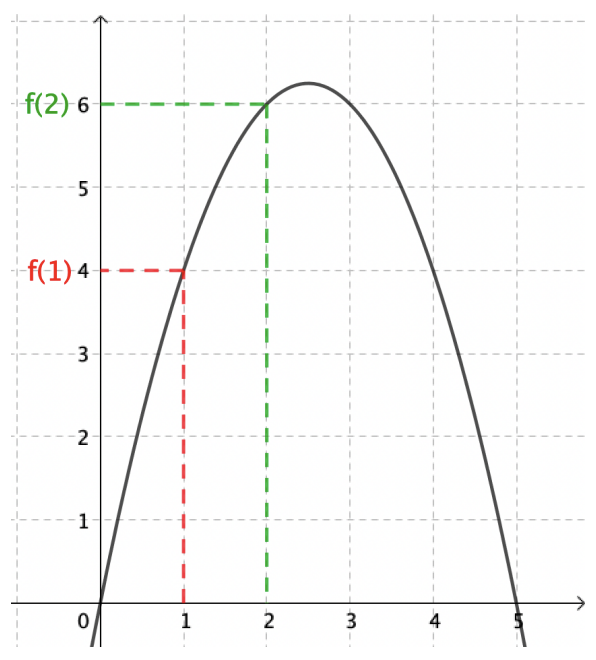
\includegraphics[width=0.8\textwidth]{var1.png}    
    \end{center}
\end{minipage}%
\hfill
\begin{minipage}[t]{.45\textwidth}%
    \vspace{0pt}
    \begin{center}
        $f$ est \_\_\_\_\_\_\_\_\_\_\_\_ sur \_\_\_\_\_\_\_

        \vspace{10pt}
        Si $x$ augmente ({\color{red}3} < {\color{ForestGreen}4}),

        \vspace{10pt}
        $f(x)$ \_\_\_\_\_\_\_\_\_\_\_\_ (\_\_\_\_\_\_\_\_\_)
        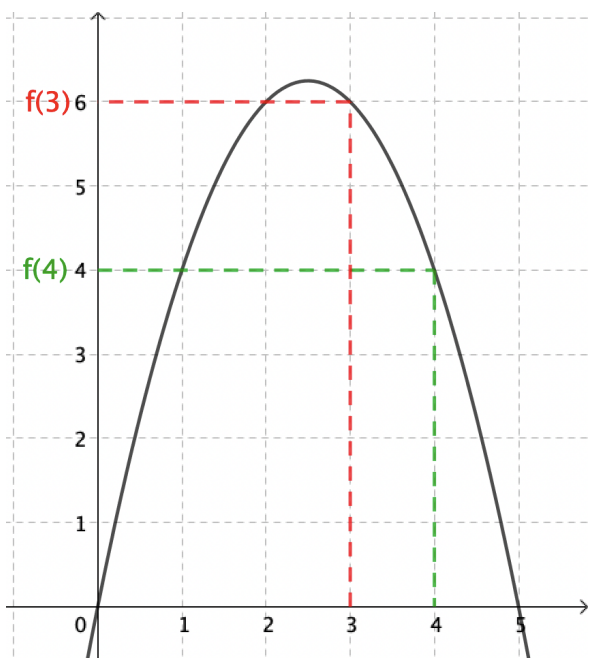
\includegraphics[width=0.8\textwidth]{var2.png}
    \end{center}
\end{minipage}%

\begin{mdframed}[
    linewidth=1pt,
    linecolor=ForestGreen,
    innertopmargin=10pt,
    innerbottommargin=10pt
]
{\color{ForestGreen}\textbf{\underline{Définition :}}}  
Sur une intervalle $I$,

\vspace{-5pt}
\begin{minipage}[t]{.45\textwidth}%
    \vspace{0pt}
    Une fonction $f$ est \textbf{croissante}, si $a < b$ alors $f(a) \leq f(b)$.
    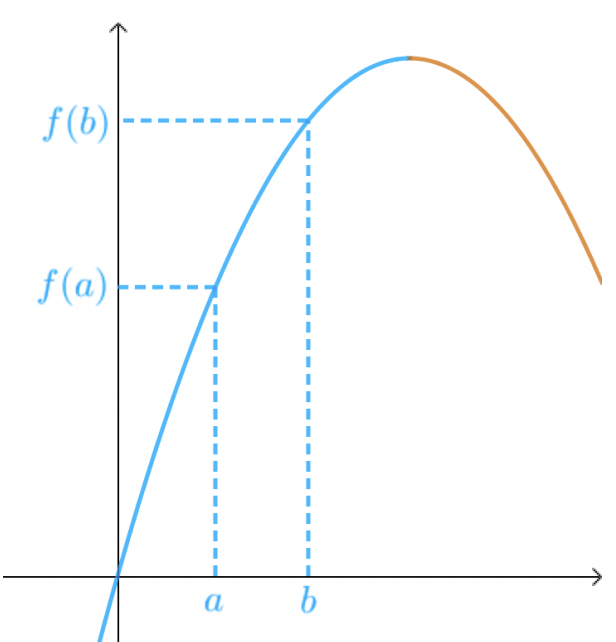
\includegraphics[width=0.8\textwidth]{vardef1.png}
\end{minipage}%
\hfill
\begin{minipage}[t]{.45\textwidth}%
    \vspace{0pt}
    Une fonction $f$ est \textbf{décroissante}, si $a < b$ alors $f(a) \geq f(b)$.
    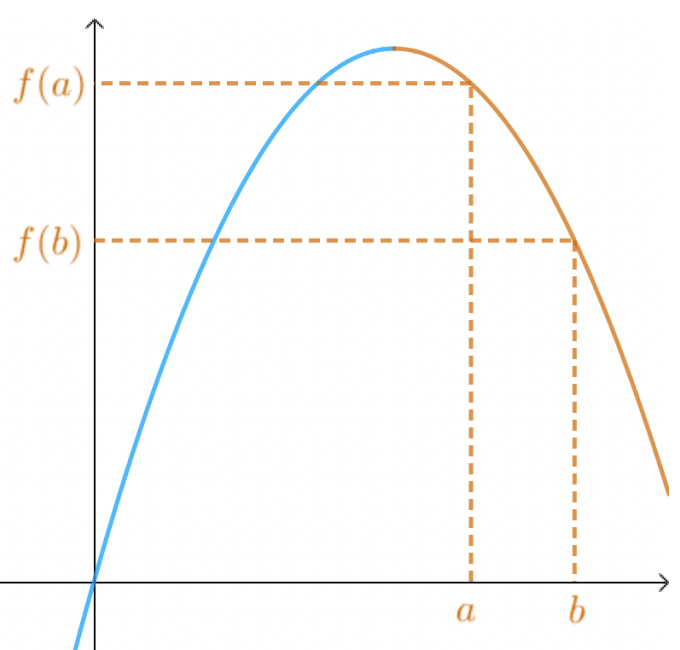
\includegraphics[width=0.8\textwidth]{vardef2.png}
\end{minipage}%
\end{mdframed}

\vspace{10pt}

\underline{Remarques :}
\begin{itemize}
    \item Pour une fonction $f$ \textbf{constante} : on a 
    toujours : \_\_\_\_\_\_\_\_\_\_\_\_.
    \item Dire que $f$ est monotone signifie que $f$ est \textbf{soit croissante soit décroissante}.
\end{itemize}

\vspace{5pt}

\begin{mdframed}[
    linewidth=1pt,
    linecolor=RoyalBlue,
    innertopmargin=10pt,
    innerbottommargin=10pt
]
{\color{RoyalBlue}\textbf{\underline{Exercice d'application n°1 :}}}
\vspace{10pt}

Décrire les variations de $g$ sur son ensemble de définition.

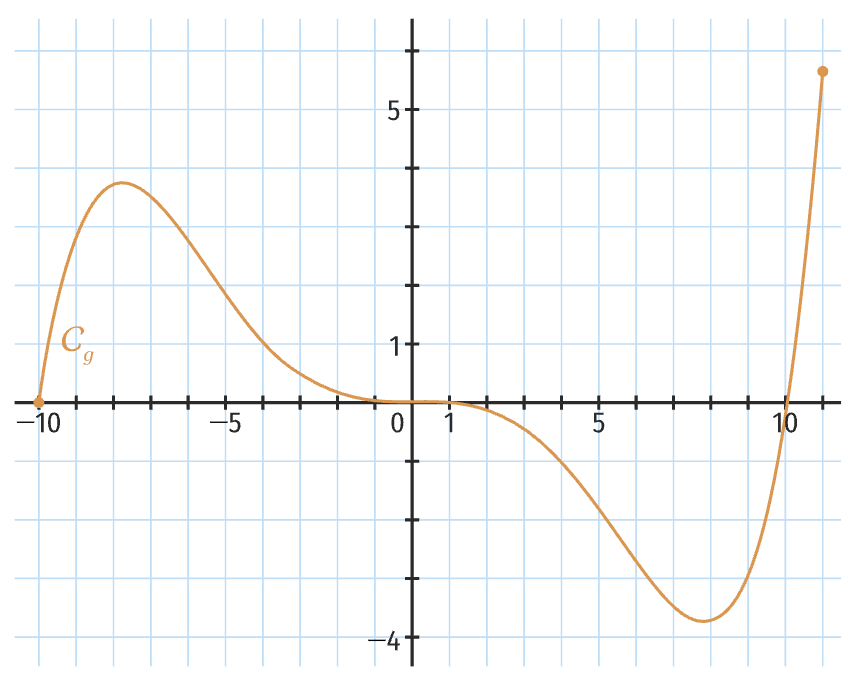
\includegraphics[width=0.6\textwidth]{exo1.png}
\end{mdframed}

\vspace{10pt}

% ========================================================
%             2) Maximum et minimum
% ========================================================
\subsection*{\hspace{1cm} 2) Maximum et minimum}

\vspace{5pt}
\underline{Exemple :}
Reprenon l'exemple de tout à l'heure avec $f(x) = 5x - x^2$.

\begin{minipage}[t]{.45\textwidth}%
    \vspace{15pt}
    Sur l’intervalle $\left[0 ; 5\right]$, on a :
    
    \vspace{15pt}
    $f(x) \leq $\ \ \_\_\_\_\_\_ $=$ \_\_\_\_\_\_.

    \vspace{15pt}
    On dit que \_\_\_\_\_\_ est le 
    
    \vspace{15pt}
    \_\_\_\_\_\_\_\_\_\_\_\_ de la fonction $f$.

    \vspace{15pt}
    Ce \_\_\_\_\_\_\_\_\_\_\_\_ est atteint en 
    
    \vspace{15pt}
    \_\_\_\_\_\_.
\end{minipage}%
\hfill
\begin{minipage}[t]{.45\textwidth}%
    \vspace{0pt}
    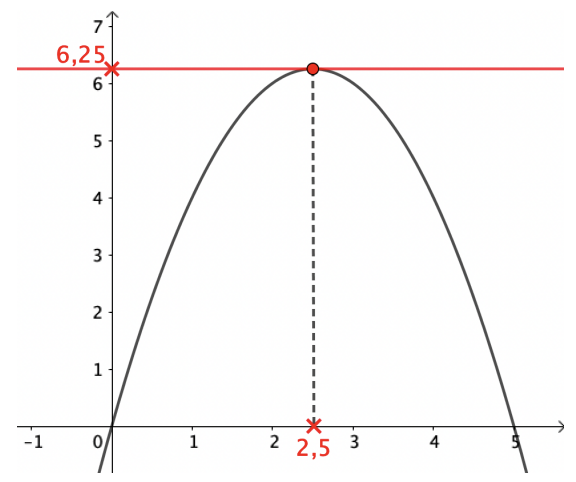
\includegraphics[width=1\textwidth]{exemple2.png}
\end{minipage}%

\begin{mdframed}[
    linewidth=1pt,
    linecolor=ForestGreen,
    innertopmargin=10pt,
    innerbottommargin=10pt
]
{\color{ForestGreen}\textbf{\underline{Définition :}}}  
Sur une intervalle $I$,

\vspace{5pt}
\begin{minipage}[t]{.45\textwidth}%
    \vspace{10pt}
    \begin{itemize}
        \item Une fonction $f$ admet un \textbf{maximum} $M$ en $a$, si pour tout $x$,
        \\$f(x) \leq f(a) = M$.

        \vspace{20pt}
        \item Une fonction $f$ admet un \textbf{minimum} $m$ en $b$, si pour tout $x$,
        \\$f(x) \geq f(b) = m$.
    \end{itemize}
\end{minipage}%
\hfill
\begin{minipage}[t]{.45\textwidth}%
    \vspace{-30pt}
    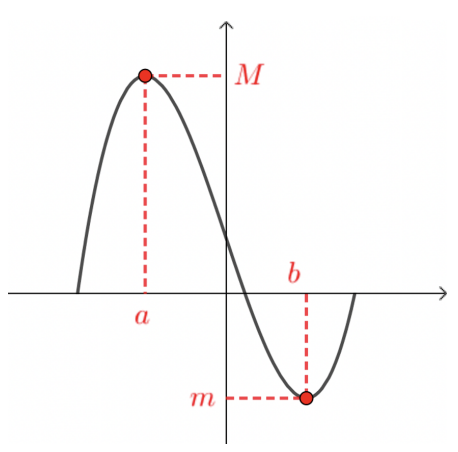
\includegraphics[width=0.8\textwidth]{defmaxmin.png}
\end{minipage}%
\end{mdframed}

\vspace{10pt}
\underline{Remarque :}
Un minimum ou un maximum s'appelle un \_\_\_\_\_\_\_\_\_\_\_\_.

\begin{mdframed}[
    linewidth=1pt,
    linecolor=RoyalBlue,
    innertopmargin=10pt,
    innerbottommargin=10pt
]
{\color{RoyalBlue}\textbf{\underline{Exercice d'application n°2 :}}}
\vspace{0pt}

\begin{minipage}[t]{.55\textwidth}%
    \vspace{0pt}
    1) $g$ admet-elle un maximum ? Un minimum ?

    \vspace{10pt}
    2) Si oui, pour quelle(s) valeur(s) de $x$ sont-ils atteints ?
\end{minipage}%
\hfill
\begin{minipage}[t]{.35\textwidth}%
    \vspace{-20pt}
    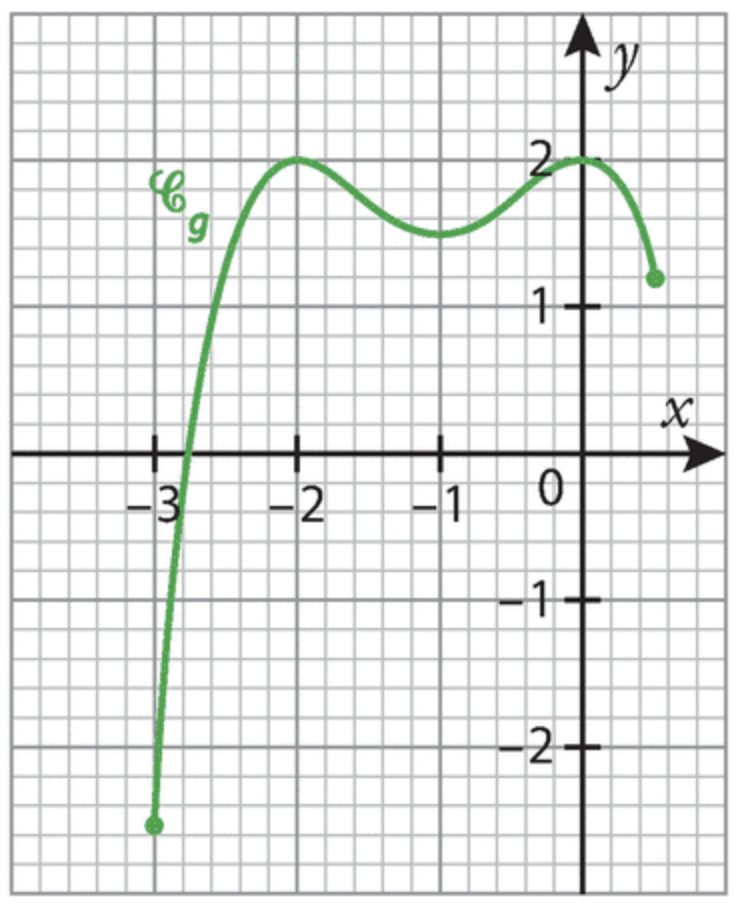
\includegraphics[width=1\textwidth]{exoextremum.png}  % Affiche l'image
\end{minipage}%

\vspace{6cm}
\end{mdframed}

\vspace{20pt}

% ========================================================
%             3) Tableau de variations
% ========================================================
\subsection*{\hspace{1cm} 3) Tableau de variations}

\vspace{5pt}
\underline{Méthode :} Déterminer graphiquement les variations d'une fonction et dresser le tableau de 
variations.

\vspace{5pt}
On considère la représentation graphique de $f$ suivante : 

\begin{center}
    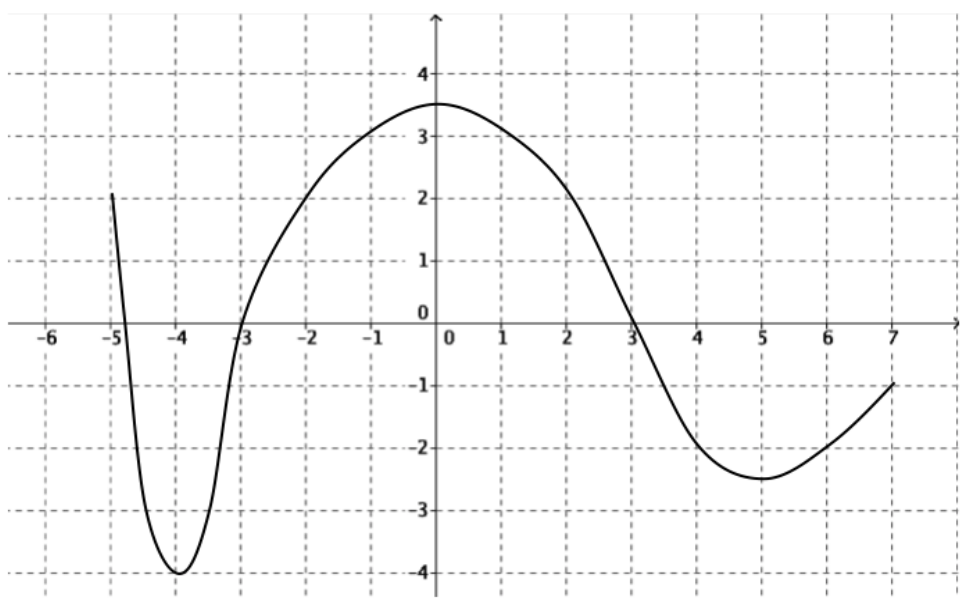
\includegraphics[width=0.8\textwidth]{exo2.png}    
\end{center}

\vspace{20pt}
La fonction $f$ est définie sur \_\_\_\_\_\_\_\_\_\_\_\_.

\vspace{20pt}
La fonction $f$ est \_\_\_\_\_\_\_\_\_\_\_\_ sur les intervalles \_\_\_\_\_\_\_\_\_\_\_\_ et \_\_\_\_\_\_\_\_\_\_\_\_.

\vspace{20pt}
Elle est \_\_\_\_\_\_\_\_\_\_\_\_ sur les intervalles \_\_\_\_\_\_\_\_\_\_\_\_ et \_\_\_\_\_\_\_\_\_\_\_\_.

\vspace{20pt}
Le maximum de $f$ est \_\_\_\_\_\_. Il est atteint en \_\_\_\_\_\_\_\_\_.

\vspace{20pt}
Le minimum de $f$ est \_\_\_\_\_\_. Il est atteint en \_\_\_\_\_\_\_\_\_ .

\vspace{20pt}
Le tableau de variation de $f$ est le suivant :
\[
\begin{tikzpicture}
    \tkzTabInit{$x$ / 1 , $f(x)$ / 2.5}
    {,,,,}
    \tkzTabLine{}
\end{tikzpicture}
\]

\newpage
\begin{mdframed}[
    linewidth=1pt,
    linecolor=RoyalBlue,
    innertopmargin=10pt,
    innerbottommargin=10pt
]
{\color{RoyalBlue}\textbf{\underline{Exercice d'application n°3 :}}}

\vspace{10pt}
On considère la fonction $f$ représentée ci-dessous.

\begin{minipage}[t]{.6\textwidth}%
    \vspace{0pt}
    1) Déterminer son maximum et la valeur en laquelle il est atteint.

    \vspace{5pt}
    2) Quel est l'ensemble de définition de la fonction ?

    \vspace{5pt}
    2) Dresser son tableau de variations.
\end{minipage}%
\hfill
\begin{minipage}[t]{.35\textwidth}%
    \vspace{-40pt}
    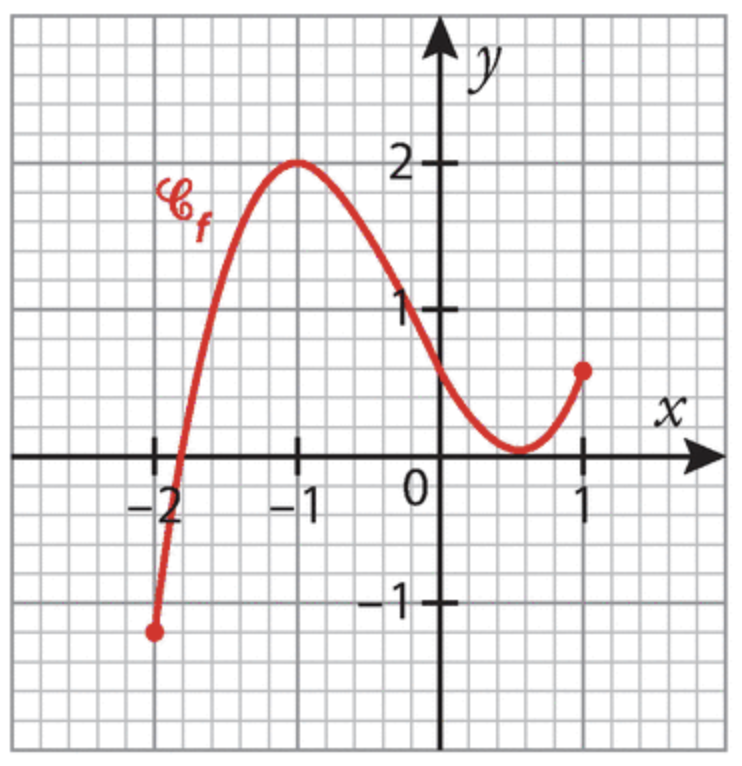
\includegraphics[draft=false,width=1\textwidth]{exo3.png}  % Affiche l'image
\end{minipage}%

\vspace{5cm}
\end{mdframed}

\vspace{20pt}
% ========================================================
%             Partie 2 : Cas des fonctions affines
% ========================================================
\section*{\textcolor{red}{Partie 2 : Cas des fonctions affines}}

% ========================================================
%             1) Définitions
% ========================================================
\subsection*{\hspace{1cm} 1) Définitions}

\begin{mdframed}[
    linewidth=1pt,
    linecolor=ForestGreen,
    innertopmargin=10pt,
    innerbottommargin=10pt
]
{\color{ForestGreen}\textbf{\underline{Définition :}}}  
Une fonction affine $f$ est définie sur $\mathbb{R}$ par $f(x) = ax+b$, où $a$ et $b$ sont deux
nombres réels.

\vspace{5pt}
Lorsque $b$ = 0, la fonction $f$ définie par $f(x) = ax$ est une fonction \_\_\_\_\_\_\_\_\_\_\_\_.
\end{mdframed}

% ========================================================
%             2) Variations
% ========================================================
\subsection*{\hspace{1cm} 2) Variations}

\begin{mdframed}[
    linewidth=1pt,
    roundcorner=5pt,
    linecolor=Red,
    innertopmargin=10pt,
    innerbottommargin=10pt
]
{\color{red}
\underline{Propriété :} \textbf{Taux d'accroissement d'une fonction affine}

\vspace{5pt}
Soit $f$ une fonction affine définie sur $\mathbb{R}$ par $f(x) = ax+b$.
\begin{itemize}
    \item Si $a>0$, alors $f$ est croissante
    \item Si $a<0$, alors $f$ est décroissante
    \item Si $a=0$, alors $f$ est constante
\end{itemize}
}
\end{mdframed}

\newpage
\underline{Méthode :}
Considérons trois fonctions $f$, $g$ et $h$ suivantes :

\begin{minipage}[t]{.25\textwidth}%
    \vspace{0pt}
    $f(x) = 3x + 2$

    \vspace{15pt}
    $g(x) = 7 - 7x$

    \vspace{15pt}
    $f(x) = -x$
\end{minipage}%
\hfill
\begin{minipage}[t]{.75\textwidth}%
    \vspace{0pt}
    $f$ est \_\_\_\_\_\_\_\_\_\_\_\_ car \_\_\_\_\_\_\_\_\_

    \vspace{15pt}
    $g$ est \_\_\_\_\_\_\_\_\_\_\_\_ car \_\_\_\_\_\_\_\_\_

    \vspace{15pt}
    $h$ est \_\_\_\_\_\_\_\_\_\_\_\_ car \_\_\_\_\_\_\_\_\_
\end{minipage}%

\vspace{20pt}
% ========================================================
%             Partie 3 : Cas des fonctions de référence
% ========================================================
\section*{\textcolor{red}{Partie 3 : Cas des fonctions de référence}}

% ========================================================
%             1) Variations de la fonction carré
% ========================================================
\subsection*{\hspace{1cm} 1) Variations de la fonction carré}

\begin{minipage}[t]{.55\textwidth}%
    \vspace{45pt}
    \begin{mdframed}[
        linewidth=1pt,
        roundcorner=5pt,
        linecolor=Red,
        innertopmargin=10pt,
        innerbottommargin=10pt
    ]
    {\color{red}
    \underline{Propriété :}

    \vspace{5pt}
    La fonction carré est \_\_\_\_\_\_\_\_\_\_\_\_ sur 
    
    \vspace{10pt}
    l'intervalle \_\_\_\_\_\_\_\_

    \vspace{10pt}
    et \_\_\_\_\_\_\_\_\_\_\_\_ sur l'intervalle \_\_\_\_\_\_
    }
    \end{mdframed}
\end{minipage}%
\hfill
\begin{minipage}[t]{.4\textwidth}%
    \vspace{0pt}
    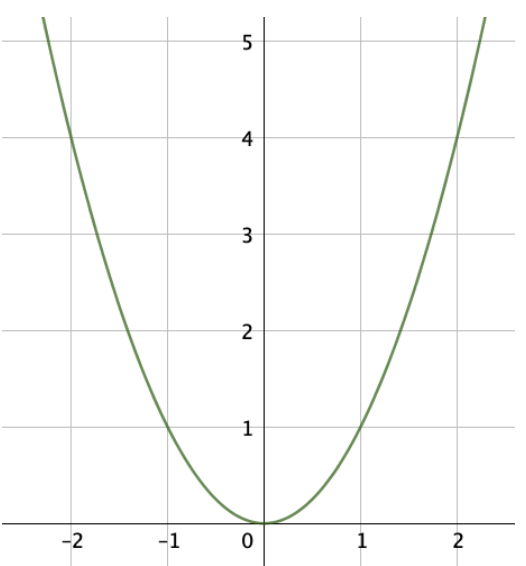
\includegraphics[width=1\textwidth]{carre.png}
\end{minipage}%

\vspace{10pt}

\begin{mdframed}[
    linewidth=1pt,
    linecolor=RoyalBlue,
    innertopmargin=10pt,
    innerbottommargin=10pt
]
{\color{RoyalBlue}\textbf{\underline{Exercice d'application n°4 :}}}

\vspace{10pt}
1) Dresser le tableau de variations de la fonction carré.

\vspace{10pt}
2) Comparer les nombres suivants sans aucun calcul :

\vspace{5pt}
\hspace{1cm}a) $2,5^2$ et $\left(\dfrac{17}{6}\right)^2$ \hspace{1cm}b) $(-3,1)^2$ et 
$\left(-\dfrac{7}{4}\right)^2$

\vspace{6cm}
\end{mdframed}

\vspace{20pt}


% ========================================================
%             2) Variations de la inverse
% ========================================================
\subsection*{\hspace{1cm} 2) Variations de la inverse}

\begin{minipage}[t]{.55\textwidth}%
    \vspace{25pt}
    \begin{mdframed}[
        linewidth=1pt,
        roundcorner=5pt,
        linecolor=Red,
        innertopmargin=10pt,
        innerbottommargin=10pt
    ]
    {\color{red}
    \underline{Propriété :}

    \vspace{5pt}
    La fonction inverse est \_\_\_\_\_\_\_\_\_\_\_\_ sur 
    
    \vspace{10pt}
    l'intervalle \_\_\_\_\_\_\_\_

    \vspace{10pt}
    et \_\_\_\_\_\_\_\_\_\_\_\_ sur l'intervalle \_\_\_\_\_\_
    }
    \end{mdframed}
\end{minipage}%
\hfill
\begin{minipage}[t]{.4\textwidth}%
    \vspace{0pt}
    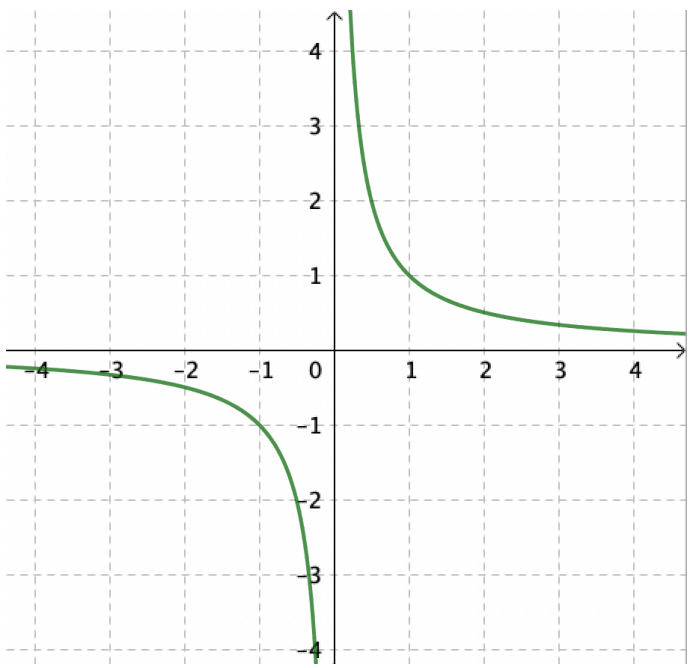
\includegraphics[width=1\textwidth]{inverse.png}
\end{minipage}%

\begin{mdframed}[
    linewidth=1pt,
    roundcorner=5pt,
    linecolor=Red,
    innertopmargin=10pt,
    innerbottommargin=10pt
]
{\color{red}
\underline{Propriété :}
Si $a$ et $b$ sont deux nombres réels de \textbf{\underline{même signe}}, on a alors :
\[
a<b \text{\ \ \ est équivalent à \ \ } \dfrac{1}{a} > \dfrac{1}{b}
\]
La fonction inverse étant \textbf{décroissante}, elle \textbf{renverse} l'ordre.
}
\end{mdframed}

\begin{mdframed}[
    linewidth=1pt,
    linecolor=RoyalBlue,
    innertopmargin=10pt,
    innerbottommargin=10pt
]
{\color{RoyalBlue}\textbf{\underline{Exercice d'application n°5 :}}}

\vspace{10pt}
1) Dresser le tableau de variations de la fonction inverse.

\vspace{10pt}
2) Comparer les nombres suivants sans aucun calcul :

\vspace{5pt}
\hspace{1cm}a) $\dfrac{1}{2,5}$ et $\dfrac{1}{3}$ \hspace{1cm}b) $\dfrac{1}{-\pi}$ et 
$\dfrac{1}{-3}$ \hspace{1cm}c) $\dfrac{1}{1,5}$ et $\dfrac{1}{\sqrt{2}}$

\vspace{6cm}
\end{mdframed}

\vspace{20pt}


% ========================================================
%             3) Variations de la fonction racine carrée
% ========================================================
\subsection*{\hspace{1cm} 3) Variations de la fonction racine carrée}

\begin{minipage}[t]{.55\textwidth}%
    \vspace{0pt}
    \begin{mdframed}[
        linewidth=1pt,
        roundcorner=5pt,
        linecolor=Red,
        innertopmargin=10pt,
        innerbottommargin=10pt
    ]
    {\color{red}
    \underline{Propriété :}

    \vspace{5pt}
    La fonction racine carré est \_\_\_\_\_\_\_\_\_\_\_\_ 
    
    \vspace{10pt}
    sur l'intervalle \_\_\_\_\_\_\_\_

    \vspace{10pt}
    et \_\_\_\_\_\_\_\_\_\_\_\_ sur l'intervalle \_\_\_\_\_\_
    }
    \end{mdframed}
\end{minipage}%
\hfill
\begin{minipage}[t]{.4\textwidth}%
    \vspace{10pt}
    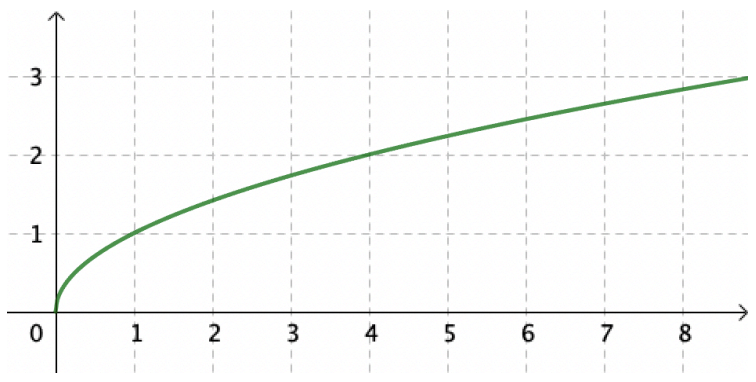
\includegraphics[width=1\textwidth]{racine.png}
\end{minipage}%

\begin{mdframed}[
    linewidth=1pt,
    roundcorner=5pt,
    linecolor=Red,
    innertopmargin=10pt,
    innerbottommargin=10pt
]
{\color{red}
\underline{Propriété :}
Si $a$ et $b$ sont deux nombres réels de \textbf{\underline{positifs}}, on a alors :
\[
a<b \text{\ \ \ est équivalent à \ \ } \sqrt{a} < \sqrt{b}
\]
La fonction racine carrée étant \textbf{croissante}, elle \textbf{conserve} l'ordre
}
\end{mdframed}

\begin{mdframed}[
    linewidth=1pt,
    linecolor=RoyalBlue,
    innertopmargin=10pt,
    innerbottommargin=10pt
]
{\color{RoyalBlue}\textbf{\underline{Exercice d'application n°6 :}}}

\vspace{10pt}
1) Dresser le tableau de variations de la fonction racine carrée.

\vspace{10pt}
2) Comparer les nombres suivants sans aucun calcul :

\vspace{5pt}
\hspace{1cm}a) $\sqrt{5}$ et $\sqrt{5,7}$ \hspace{1cm}b) $\sqrt{2}$ et 
$\sqrt{\dfrac{5}{2}}$ \hspace{1cm}c) $\sqrt{\dfrac{10}{3}}$ et $\sqrt{2,7}$

\vspace{7cm}
\end{mdframed}

\vspace{20pt}


% ========================================================
%             4) Variations de la fonction cube
% ========================================================
\subsection*{\hspace{1cm} 4) Variations de la fonction cube}

\begin{minipage}[t]{.55\textwidth}%
    \vspace{25pt}
    \begin{mdframed}[
        linewidth=1pt,
        roundcorner=5pt,
        linecolor=Red,
        innertopmargin=10pt,
        innerbottommargin=10pt
    ]
    {\color{red}
    \underline{Propriété :}

    \vspace{5pt}
    La fonction cube est \_\_\_\_\_\_\_\_\_\_\_\_ sur 
    
    \vspace{10pt}
    l'intervalle \_\_\_\_\_\_\_\_

    \vspace{10pt}
    et \_\_\_\_\_\_\_\_\_\_\_\_ sur l'intervalle \_\_\_\_\_\_
    }
    \end{mdframed}
\end{minipage}%
\hfill
\begin{minipage}[t]{.35\textwidth}%
    \vspace{-10pt}
    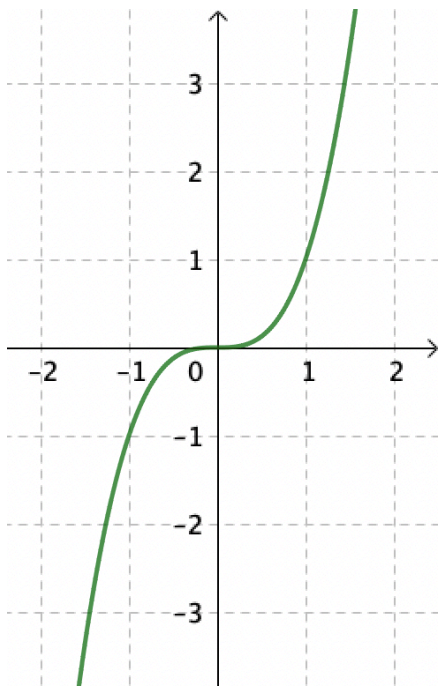
\includegraphics[width=0.8\textwidth]{cube.png}
\end{minipage}%

\begin{mdframed}[
    linewidth=1pt,
    roundcorner=5pt,
    linecolor=Red,
    innertopmargin=10pt,
    innerbottommargin=10pt
]
{\color{red}
\underline{Propriété :}
Si $a$ et $b$ sont deux nombres réels de \textbf{\underline{positifs}}, on a alors :
\[
a<b \text{\ \ \ est équivalent à \ \ } a^3 < b^3
\]
La fonction cube étant \textbf{croissante}, elle \textbf{conserve} l'ordre
}
\end{mdframed}

\begin{mdframed}[
    linewidth=1pt,
    linecolor=RoyalBlue,
    innertopmargin=10pt,
    innerbottommargin=10pt
]
{\color{RoyalBlue}\textbf{\underline{Exercice d'application n°7 :}}}

\vspace{10pt}
1) Dresser le tableau de variations de la fonction cube.

\vspace{10pt}
2) Comparer les nombres suivants sans aucun calcul :

\vspace{5pt}
\hspace{1cm}a) $2,5^3$ et $4^3$ \hspace{1cm}b) $(-4)^3$ et 
$(-7)^3$ \hspace{1cm}c) $\left(\dfrac{5}{9}\right)^3$ et $\left(\dfrac{8}{7}\right)^3$

\vspace{7cm}
\end{mdframed}

\vspace{20pt}











\end{document}
